% =====================================================================
%  PAPER B — the QuickReview technical report. Companion: benchmark.tex
%  (the benchmark paper), which every evaluation number here comes from.
%
%  DRAFT (2026-09-28; base model, stability and the current-build re-run
%  added 2026-09-30; rewritten 2026-10-01 around the final comparison:
%  every contender at the best configuration found for it, all
%  OpenAI-based reviewers on gpt-6.1-sol). Single file: diagrams are
%  TikZ, the bibliography is inline (no bibtex run needed).
%  Every number is copied from bench/aacr/FULL-BENCHMARK.md,
%  docs/METHODOLOGY.md, docs/THREATS-TO-VALIDITY.md, METRICS.md,
%  RESULTS.md or charts/numbers*.json unless a footnote says otherwise.
%  Gap markers:
%    \NEEDDATA  -- a number we could compute from existing runs/files
%    \NEEDEXP   -- an experiment we have not run
%    \TODO      -- editorial work
% =====================================================================
\documentclass[11pt,a4paper]{article}

\usepackage[utf8]{inputenc}
\usepackage[T1]{fontenc}
\usepackage{lmodern}
\usepackage[margin=2.5cm]{geometry}
\usepackage{booktabs}
\usepackage{graphicx}
\usepackage{xcolor}
\usepackage{array}
\usepackage{tabularx}
\usepackage{amsmath}
\usepackage{enumitem}
\usepackage{tikz}
\usetikzlibrary{arrows.meta,positioning,fit,calc,backgrounds,shapes.geometric}
\usepackage[hidelinks]{hyperref}

\newcommand{\NEEDDATA}[1]{\textcolor{red}{\textbf{[NEED DATA: #1]}}}
\newcommand{\NEEDEXP}[1]{\textcolor{orange}{\textbf{[NEED EXPERIMENT: #1]}}}
\newcommand{\TODO}[1]{\textcolor{blue}{\textbf{[TODO: #1]}}}

\newcommand{\qcr}{QuickReview}
\newcommand{\code}[1]{\texttt{#1}}
\newcommand{\chart}[1]{../charts/#1.jpg}

% diagram styles
\tikzset{
  box/.style={draw, rounded corners=2pt, align=center, font=\small,
    inner sep=4pt, minimum height=2.2em, fill=white},
  agent/.style={box, fill=blue!6},
  data/.style={box, fill=gray!8, sharp corners},
  human/.style={box, fill=orange!10},
  judge/.style={box, fill=green!8},
  flow/.style={-{Stealth[length=2mm]}, thick},
  note/.style={font=\footnotesize\itshape, align=center, text=black!70},
}

\setlist{itemsep=2pt,topsep=4pt}
\setlength{\emergencystretch}{3em}

\title{QuickReview: a multi-pass automated code reviewer,\\
\large and how it performs on a verified defect benchmark}
\author{\TODO{authors and affiliation} \\ Quickchat AI}
\date{Draft of 2026-10-01}

\begin{document}
\maketitle

\begin{abstract}
QuickReview is an automated pull-request reviewer built as a multi-pass
system: for every PR one main session launches about eleven independent
lens passes chosen from the change --- a baseline, a tests lens, a sweep
over every changed file, code-quality lenses and content-triggered
sub-lenses --- and a validator then re-derives every candidate finding
from the code before one review is posted. This report describes the
design and measures it on a verified defect benchmark for AACR-Bench
built in a companion paper~\cite{qcrbench}. With every OpenAI-based
reviewer on gpt-6.1-sol and each third-party tool at the best
configuration found for it, QuickReview's default preset finds 409 of 520
verified defects (79\%, 95\% interval 75--82\%) with 95\% of its comments
correct; its low-effort preset finds 70\%, the strongest third-party
configuration (pi-review's three-reviewer panel) 67\%, and Claude Code on
Claude Opus 5.5 62\%. The lead is in medium- and low-severity defects; on
the 90 high-severity defects QuickReview, pi-review's panel and Codex CLI
are not separated. It is also the most expensive reviewer, at \$1.36 per
PR against \$0.07--\$0.53, and we show where the cost goes: redundant
independent lenses that re-derive the same defects, and a validator that
checks every candidate. Holding the harness fixed and changing only the
model moves its recall from 28\% (gpt-6-luna) to 84\% (gpt-6-sol) on 185
PRs and to 95\% (Claude Opus 5.5) on 40. A full re-run reproduced the
result within 1.5 defects. Because the benchmark was built by the same
team, partly from QuickReview's own earlier output, we state where that
could inflate these numbers.
\end{abstract}


\tableofcontents
\clearpage

% =====================================================================
\section{Introduction}
\label{sec:intro}

QuickReview\footnote{Its code, configuration and earlier reports call it
\code{quickreviewd}.} is the automated reviewer we run on our own
repositories: a daemon receives pull-request events, and for every
triggered PR a reviewing session writes one review, with inline comments,
a verdict and a section of points for a human to double-check. We wanted
to know whether it finds the problems a careful senior reviewer would
raise before merge, how it compares with the review tools a team could
adopt instead, and what its design buys for what it costs.

Answering that needed a benchmark that counts real defects, which we
built and describe in a companion paper~\cite{qcrbench}: a verified
answer key of 520 defects over the 185 runnable PRs of
AACR-Bench~\cite{aacrbench}, a defect-level judge checked across two model
families, and a protocol that gives every competing tool the best
configuration its own documentation ships or recommends. This report is
about the reviewer. Section~\ref{sec:benchbrief} summarises the benchmark;
Section~\ref{sec:design} describes QuickReview's design;
Section~\ref{sec:qresults} gives its results against seven other
reviewers; Section~\ref{sec:discussion} explains its cost and compares it
with the closest competitor design; Section~\ref{sec:basemodel} changes
only its base model; Section~\ref{sec:stabsec} measures how stable its
result is; and Section~\ref{sec:limits} lists what these numbers do not
show, starting with the fact that the benchmark's authors also built this
reviewer.

% =====================================================================
\section{The benchmark in brief}
\label{sec:benchbrief}

\begin{figure}[t]
\centering
\resizebox{\textwidth}{!}{%
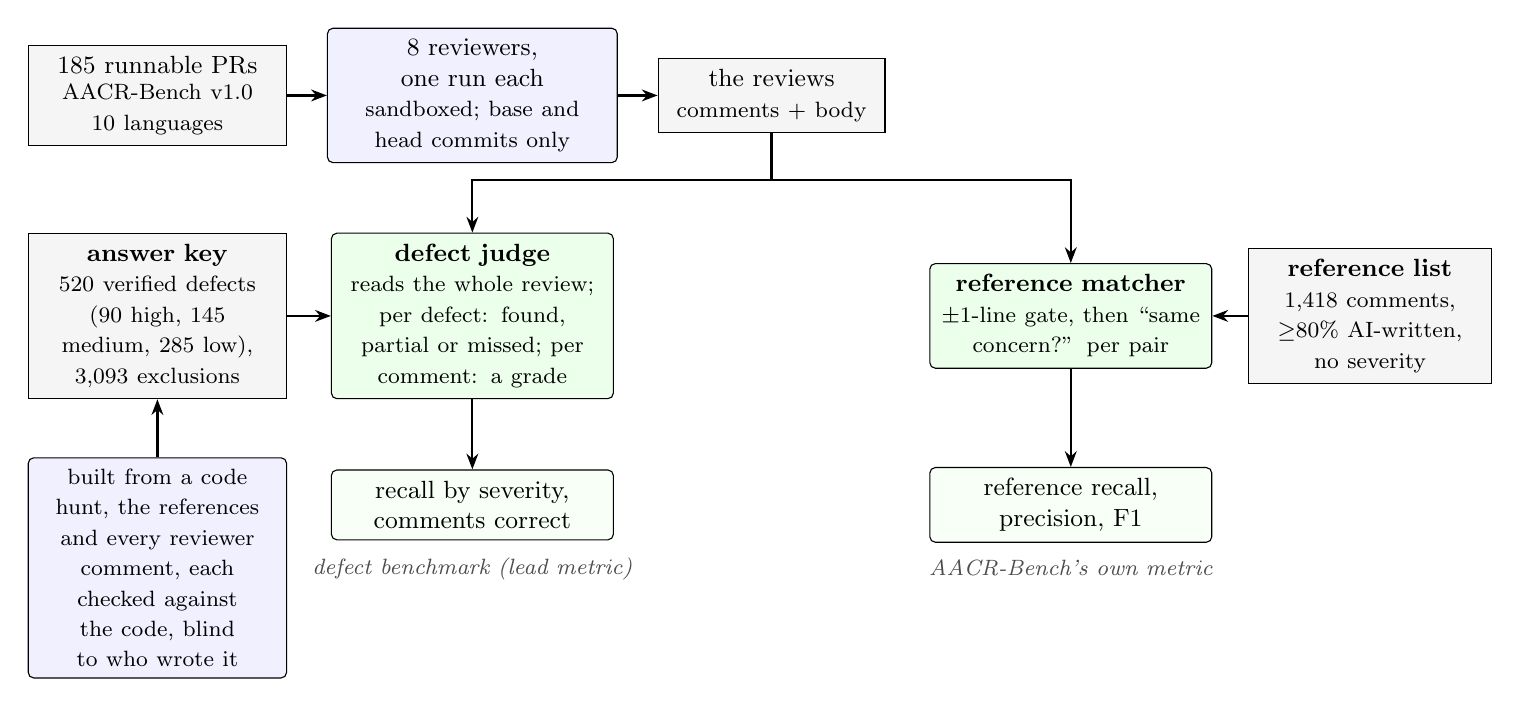
\begin{tikzpicture}
  \node[data, text width=3.0cm] (prs) at (0,0) {185 runnable PRs\\ \footnotesize AACR-Bench v1.0\\ 10 languages};
  \node[agent, text width=3.4cm] (rev) at (4.0,0) {8 reviewers, one run each\\ \footnotesize sandboxed; base and head commits only};
  \node[data, text width=2.6cm] (out) at (7.8,0) {the reviews\\ \footnotesize comments + body};
  \draw[flow] (prs) -- (rev);
  \draw[flow] (rev) -- (out);

  \node[judge, text width=3.3cm] (dj) at (4.0,-2.8) {\textbf{defect judge}\\ \footnotesize reads the whole review; per defect: found, partial or missed; per comment: a grade};
  \node[judge, text width=3.3cm] (aj) at (11.6,-2.8) {\textbf{reference matcher}\\ \footnotesize $\pm1$-line gate, then ``same concern?'' per pair};
  \draw[flow] (out.south) -- ++(0,-0.6) -| (dj.north);
  \draw[flow] (out.south) -- ++(0,-0.6) -| (aj.north);

  \node[data, text width=3.0cm] (key) at (0,-2.8) {\textbf{answer key}\\ \footnotesize 520 verified defects (90 high, 145 medium, 285 low), 3{,}093 exclusions};
  \node[data, text width=2.8cm] (refs) at (15.4,-2.8) {\textbf{reference list}\\ \footnotesize 1{,}418 comments, $\ge$80\% AI-written, no severity};
  \draw[flow] (key) -- (dj);
  \draw[flow] (refs) -- (aj);

  \node[box, fill=green!3, text width=3.3cm] (m1) at (4.0,-5.2) {recall by severity,\\ comments correct};
  \node[box, fill=green!3, text width=3.3cm] (m2) at (11.6,-5.2) {reference recall,\\ precision, F1};
  \draw[flow] (dj) -- (m1);
  \draw[flow] (aj) -- (m2);
  \node[note, below=1mm of m1] {defect benchmark (lead metric)};
  \node[note, below=1mm of m2] {AACR-Bench's own metric};

  \node[agent, text width=3.0cm] (gt) at (0,-6.0) {\footnotesize built from a code hunt, the references and every reviewer comment, each checked against the code, blind to who wrote it};
  \draw[flow] (gt) -- (key);
\end{tikzpicture}}
\caption{How the benchmark works. Every review is scored twice: by our
defect judge against a verified answer key (left; the lead metric) and by AACR-Bench's own reference-comment metric (the
benchmark's published score). The companion paper~\cite{qcrbench} builds the key and the judge.}
\label{fig:howitworks}
\end{figure}


Each of the 185 runnable PRs of AACR-Bench v1.0 carries a list of
verified defects --- 520 in all, 90 high, 145 medium and 285 low severity
--- built by a code hunt, the dataset's reference comments and the
benchmarked reviewers' comments, each candidate checked against the code
by agents that could not see who raised it, with 3{,}093 rejected
candidates kept with their reasons. A judge model reads each review whole
and grades every defect found, partly found (counted as half) or missed,
and every comment correct-valuable, correct-minor, partly correct or
incorrect. Two judges from different model families agreed on 98.7\% of
verdicts. Every reviewer runs in a locked-down container that sees only
the PR's base and head commits. The full method, its rejected
alternatives and its threats are in the companion paper~\cite{qcrbench};
two of those threats bear on QuickReview directly and are repeated in
Section~\ref{sec:limits}.

% =====================================================================
\section{Design}
\label{sec:design}

Three choices shape QuickReview. \emph{Independent angles}: a review is
the union of many narrow passes rather than one long read, each pass a
leaf session that starts from the diff and the code and does not see the
others, so a defect one pass misses is often re-derived by another.
\emph{A check before posting}: a validator re-derives every candidate from
the code and posts, merges, demotes or doubts it; since its veto
is a mark rather than a deletion, so a cheaper validator cannot make a
stronger lens's finding disappear. \emph{Read, never run}: the reviewer
reads code and CI results and never executes code; anything that needs
execution is CI's job. The production system adds what a benchmark
cannot see --- reviewer memory, CI gating of approvals, rechecks after
approval --- and those are off in every number here.

\subsection{One round}

\qcr{} runs one main session per PR. The session receives a round order
listing a pass plan: lenses chosen from the diff (for example baseline,
simplicity, widened checks, tests, maintainability, duplication,
abstraction, consistency, a per-file sweep) and a validator that runs
last and kills or demotes candidate findings the code refutes. The
session may add lenses but never drop a planned one. Passes are leaves
(no nested fan-out). The \code{default} preset enables the
benchmark-driven levers from the tuning phase (content-triggered
sub-lenses, the per-file sweep, dependency sources unpacked at their
locked versions, the validator's ``restate, don't kill'' and ``demote,
don't kill'' rules) with the lean plan, and the code-quality lenses
(capped below blocking; style only against a repository's written
guide). Figure~\ref{fig:round} shows one round.
Over the 185 PRs of the earlier gpt-6-sol run, default ran a mean of
11.2 passes per PR
(validator included; median 11, interquartile range 9--14, range 4--24)
and low 11.0 (the same median, quartiles and range). The plans are the
same size, 10.9 on average, because the presets change model tiers, not
the plan. The session added passes beyond the plan on 36 PRs under
default and 18 under low. Every PR ran baseline, tests, the per-file
sweep and the validator. The four code-quality lenses ran on 77\% of PRs,
simplicity on 65\%, intent on 45\%, and every other lens on 39\% or
fewer.\footnote{Computed from \code{executed\_passes} and
\code{planned\_lenses} in each case's \code{case-summary.json}, for the
runs in \code{FULL-BENCHMARK.md}, 2026-09-29.}


\begin{figure}[t]
\centering
\resizebox{\textwidth}{!}{%
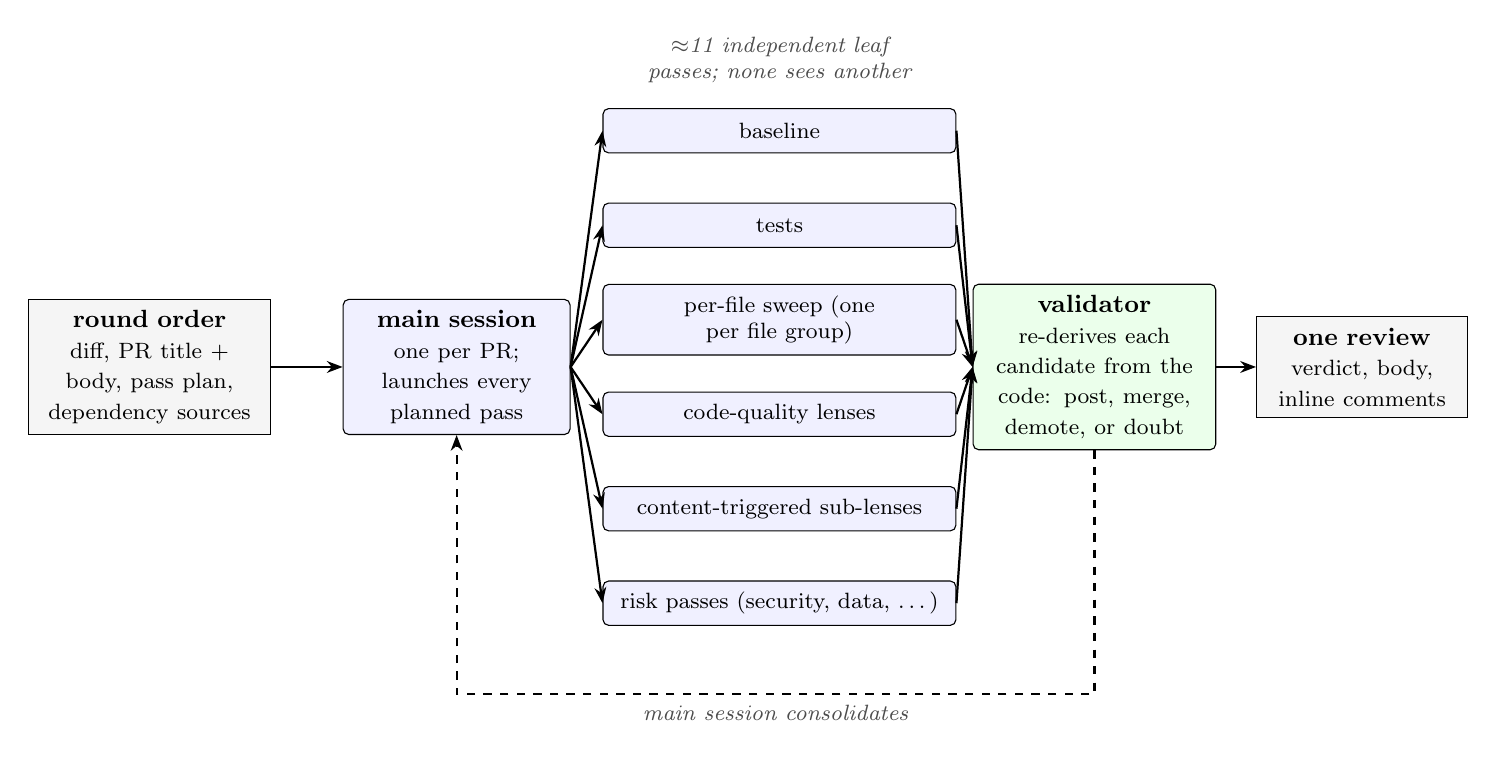
\begin{tikzpicture}
  \node[data, text width=2.8cm] (in) at (0,0) {\textbf{round order}\\ \footnotesize diff, PR title + body, pass plan, dependency sources};
  \node[agent, text width=2.6cm] (main) at (3.9,0) {\textbf{main session}\\ \footnotesize one per PR; launches every planned pass};
  \foreach \i/\y/\t in {1/3.0/baseline, 2/1.8/tests, 3/0.6/per-file sweep (one per file group), 4/-0.6/code-quality lenses, 5/-1.8/content-triggered sub-lenses, 6/-3.0/{risk passes (security, data, \ldots)}} {
    \node[agent, text width=4.2cm, minimum height=1.6em, font=\footnotesize] (L\i) at (8.0,\y) {\t};
    \draw[flow] (main.east) -- (L\i.west);
  }
  \node[note, text width=4.6cm] at (8.0,3.9) {$\approx$11 independent leaf passes; none sees another};
  \node[judge, text width=2.8cm] (val) at (12.0,0) {\textbf{validator}\\ \footnotesize re-derives each candidate from the code: post, merge, demote, or doubt};
  \foreach \i in {1,...,6} { \draw[flow] (L\i.east) -- (val.west); }
  \node[data, text width=2.4cm] (rev) at (15.4,0) {\textbf{one review}\\ \footnotesize verdict, body, inline comments};
  \draw[flow] (in) -- (main);
  \draw[flow] (val) -- (rev);
  \draw[flow, dashed] (val.south) -- ++(0,-3.1) -| node[note, pos=0.25, below] {main session consolidates} (main.south);
\end{tikzpicture}}
\caption{One \qcr{} round. The main session launches every planned
pass as an isolated leaf (no nested fan-out) and may add passes, never drop
one; the validator runs last at high reasoning. Of the default's cost on
the earlier 185-PR run, the passes took 75.5\%, the validator 10.9\% and
the main session 13.5\% (Section~\ref{sec:whycost}).}
\label{fig:round}
\end{figure}


\subsection{Presets}
\label{sec:presets}

One configuration word sets the whole round. \code{default} enables every
lever from the tuning phase (content-triggered sub-lenses, the per-file
sweep, dependency sources unpacked at their locked versions, the
validator's ``restate, don't kill'' and ``demote, don't kill'' rules)
with the lean plan, lenses at medium reasoning and the validator and risk
passes at high. \code{low} keeps the same plan with every model at low
reasoning, for about two thirds of the cost. \code{max} puts every model
at its ceiling and runs the full lever plan; it was measured only as an
anecdote (Section~\ref{sec:basemodel}). An explicitly set key always
overrides the preset.

\subsection{How it runs on the benchmark}

The benchmark runs the production round, not a benchmark build: the real
round order, session system prompt, lens and validator agents and model
configuration. The main difference is a \textsc{benchmark mode} section
appended to the round order, which says there is no GitHub, no CI and no
memory, and tells the session to write its would-be review to files
instead of posting it. Memory is off, so a foreign repository never
reads or writes the production reviewer's memory; a multi-line comment is
scored at its single anchor line. A benchmark-tuned switch that posts
every true nit (\code{[review] nits = "open"}) exists because AACR's
metric rewards nits; it was measured and is off in every scored run.

% =====================================================================
\section{Results on the benchmark}
\label{sec:qresults}

Eight reviewers ran once each on all 185 PRs: QuickReview's
\code{default} and \code{low} presets and six third-party tools ---
pi-review~\cite{pireview}, Claude Code~\cite{claudecode},
open-code-review~\cite{ocr}, Codex CLI~\cite{codex},
OpenCode~\cite{opencode} and PR-Agent~\cite{pragent} --- each in
the best configuration found for it among the variants its own
documentation ships or recommends, chosen by a rule fixed in advance on
40 PRs~\cite{qcrbench}. Every OpenAI-based reviewer ran on gpt-6.1-sol;
Claude Code ran on Claude Opus 5.5.

\begin{table}[t]
  \centering
  \caption{The final comparison: defect benchmark, 185 PRs, 520 defects,
  primary judge. A partly found defect counts $\tfrac12$. Weighted recall:
  high 3, medium 2, low 1. \$ are list prices, not bills (gpt-6.1-sol at
  \$2 / \$0.10 / \$10 per million uncached input / cached input / output
  tokens; Claude Code its own reported cost).\protect\footnotemark}
  \label{tab:final}
  \resizebox{\textwidth}{!}{%
  \begin{tabular}{lrrrrrrrrr}
    \toprule
    Reviewer & Found & Recall & High (90) & Med.\ (145) & Low (285) & Weighted & Correct & \$/PR & Median min/PR \\
    \midrule
    \textbf{\qcr{} default} & \textbf{409} & \textbf{79\%} & \textbf{83.5} & \textbf{121} & \textbf{204.5} & \textbf{82\%} & \textbf{95\%} & 1.36 & 9.5 \\
    \qcr{} low & 365.5 & 70\% & 79.5 & 104.5 & 181.5 & 74\% & 94\% & 0.88 & 6.7 \\
    pi-review panel (high) & 347.5 & 67\% & 80 & 119 & 148.5 & 74\% & 89\% & 0.27 & 1.8 \\
    Claude Code (Opus 5.5) & 324.5 & 62\% & 72.5 & 105 & 147 & 68\% & 81\% & 0.20 & 0.7 \\
    open-code-review high & 298.5 & 57\% & 63.5 & 102 & 133 & 62\% & 86\% & 0.53 & 1.8 \\
    Codex CLI high & 287 & 55\% & 81 & 101.5 & 104.5 & 65\% & 93\% & 0.14 & 2.1 \\
    OpenCode native + PR text & 263.5 & 51\% & 76 & 99 & 88.5 & 61\% & 93\% & 0.17 & 2.3 \\
    PR-Agent & 194 & 37\% & 55.5 & 70 & 68.5 & 44\% & 76\% & 0.07 & 1.9 \\
    \bottomrule
  \end{tabular}}
\end{table}
\footnotetext{\code{compare.py -{}-cases all30+fresh10+rest145} on the runs
listed in \code{bench/aacr/final/arms.txt}; reproduced independently from
the judge files, 2026-10-01.}


\begin{figure}[t]
  \centering
  \includegraphics[width=\textwidth]{\chart{defects-by-severity}}
  \caption{The final comparison: real defects found, split by severity
  (dark: high, mid: medium, light: low), 185 PRs, primary judge.}
  \label{fig:sev}
\end{figure}

The default finds 409 of the 520 defects (79\%) with 95\% of its comments
correct (Table~\ref{tab:final}, Figure~\ref{fig:sev}). Its lead over every
other reviewer on overall recall excludes zero in a paired bootstrap over
PRs: $+8.4$ points over \code{low}, $+11.8$ [$+7.8$, $+15.7$] over
pi-review's panel, $+16.2$ over Claude Code. It is a lead in medium and
above all low severity: on the 90 high-severity defects the default finds
83.5, Codex CLI 81, the panel 80 and \code{low} 79.5, and none of those
gaps is established. On medium severity the default and the panel are
level (121 and 119 of 145); on low severity the default finds 204.5 of
285 against 148.5.

\begin{table}[t]
  \centering
  \small
  \caption{Recall, high-severity recall and weighted recall with 95\%
  bootstrap intervals over PRs (seed 20261001), and cost per defect found
  (total list cost over the 185 PRs divided by problems found).}
  \label{tab:ci}
  \resizebox{\textwidth}{!}{%
  \begin{tabular}{lrrrrr}
    \toprule
    Reviewer & Recall [95\% CI] & High recall [95\% CI] & Weighted [95\% CI] & \$/defect & \$/high defect \\
    \midrule
    \qcr{} default & 78.7\% [74.8, 82.2] & 92.8\% [87.2, 97.4] & 82.5\% [79.1, 85.6] & 0.61 & 3.01 \\
    \qcr{} low & 70.3\% [66.2, 74.1] & 88.3\% [81.0, 94.7] & 74.4\% [70.5, 78.2] & 0.44 & 2.04 \\
    pi-review panel (high) & 66.8\% [63.3, 70.4] & 88.9\% [82.8, 94.9] & 74.1\% [70.8, 77.4] & 0.14 & 0.62 \\
    Claude Code (Opus 5.5) & 62.4\% [58.6, 66.4] & 80.6\% [71.1, 89.6] & 68.0\% [64.0, 72.1] & 0.11 & 0.50 \\
    open-code-review high & 57.4\% [51.9, 62.5] & 70.6\% [58.8, 82.0] & 62.4\% [56.2, 68.1] & 0.33 & 1.55 \\
    Codex CLI high & 55.2\% [51.0, 59.0] & 90.0\% [83.8, 95.5] & 65.1\% [61.4, 68.6] & 0.09 & 0.33 \\
    OpenCode native + PR text & 50.7\% [47.1, 54.4] & 84.4\% [77.6, 90.8] & 60.9\% [57.3, 64.4] & 0.12 & 0.42 \\
    PR-Agent & 37.3\% [33.7, 41.1] & 61.7\% [51.2, 72.5] & 44.4\% [40.1, 48.7] & 0.06 & 0.22 \\
    \bottomrule
  \end{tabular}}
\end{table}

\paragraph{What it says.} The default posts the most comments (5.4 per
PR) and has the fewest graded incorrect (2.5\%), but a third of them are
true and minor, and only 56\% map to a verified defect, against 81--87\%
for Claude Code, Codex CLI and OpenCode. It finds more, and says more.

\paragraph{Where it was tuned and where it was not.} QuickReview's levers
were designed from its misses on the original 40 PRs; the other 145 were
never looked at before its final build. It scores lower on the 40 (70\%)
than on the 145 (81\%), and so does every other reviewer, so the 40 are
harder for everyone; its margin over the mean of the other seven is 18.2
points on the 40 and 22.5 on the 145, the opposite of what tuning on the
40 would produce. On the 369 defects the key would hold without any
reviewer's comment it finds 81\%, against 74\% for \code{low} and 69--70\%
for the panel and Claude Code.

\paragraph{By kind.} The largest margin is on maintainability defects
(81\% against 16--51\% for the third-party tools), which fits the
code-quality lenses; those lenses were designed on the tuning PRs, so it
is also where a design-to-key alignment would show first. Without the 72
maintainability defects the default finds 78\% against 71\% for the panel.

\paragraph{Worked examples.} The companion paper~\cite{qcrbench} shows one
defect of each severity with every reviewer's verdict and comments,
including a medium-severity defect that five other reviewers found and
QuickReview found only in part.

% =====================================================================
\section{Why it costs more, and the closest competitor}
\label{sec:discussion}

\subsection{Why \qcr{} costs more}
\label{sec:whycost}

\qcr{} spends more per PR than any other tool because of how it is built,
and on this benchmark that spending is what buys its recall.

\paragraph{Redundant coverage by independent lenses.} A round runs about 11
passes (11.2 per PR on average under default, validator included;
the benchmark paper~\cite{qcrbench}): lenses that each examine the same change from a
different angle. Each lens is a separate subagent that starts from the diff
and the code; the lenses do not see or talk to each other. The overlap is
large and deliberate. Of the 440 defects credited to the default arm on the
185 PRs, only 71 were raised by a single lens, and 127 by six or more (two
lenses 57, three 72, four 60, five 53). A defect that one lens misses is
usually re-derived independently by another.\footnote{Per-lens attribution
over the default arm's findings records, re-derived by an independent
verifier; tuning analysis of 2026-09-30.}

\paragraph{An adversarial validator.} After the lenses, a separate validator
pass at high reasoning re-checks every candidate against the code and
posts, merges, demotes or kills it. On the 185-PR default run it handled
2{,}959 candidates: 1{,}456 merged as duplicates of another finding (the
redundancy above, collapsed), 1{,}034 posted, 164 demoted and posted, 207
killed (a kill rate of 7.0\%), 64 withheld and 34 folded. Hand-checking the
kills found about 6 of the 520 real defects wrongly killed, about 1.2 points
of recall. The main session then consolidates what survives into one
review. The cross-examination is independent re-derivation followed by a
verifier, not a discussion between lenses. Of the default's cost, the
lenses take 75.5\%, the validator 10.9\% and the main session 13.5\%.

\paragraph{What the compute buys.} In the final comparison \qcr{}'s
default has both the highest recall (79\%) and the highest share of
correct comments (95\%); the other tools reach 37--67\% with 76--93\% of
their comments correct (Table~\ref{tab:final}). With the harness fixed,
less compute finds less: the \code{low} preset finds 70\% at \$0.88 per PR
against 79\% at \$1.36, and a small base model that writes about half as
much per pass collapses to 28\% (Section~\ref{sec:basemodel}). The lenses
are not interchangeable copies either: on the earlier 185-PR default run
the per-file sweep alone was the only route to 29 credited defects (2
high), and dropping it is estimated to cost about 5.6 points of recall.

\paragraph{The counterpoint.} \qcr{}'s case is recall, not cost
efficiency. In the final comparison every other tool is cheaper per PR,
by 2.6 times (open-code-review, \$0.53) to 21 times (PR-Agent, \$0.07),
and cheaper per defect found: \$0.06--\$0.14 for PR-Agent, Codex CLI,
Claude Code, OpenCode and pi-review's panel against \$0.61 for the default
(Table~\ref{tab:ci}). On high-severity defects alone the default's lead
over the panel and Codex CLI is not established, and they find a
high-severity defect for \$0.62 and \$0.33 against \$3.01. A team that
wants the most important findings cheaply is better served by one of those
tools at its best configuration; \qcr{} is the choice when a missed
medium- or low-severity defect costs more than the review.

\subsection{Why pi-review's panel is the strongest competitor}
\label{sec:panel}

Of every third-party configuration we ran, pi-review's three-reviewer panel
comes closest to \qcr{}, and it is also the one whose design is closest to
\qcr{}'s. In the final comparison it finds 347.5 of 520 defects (67\%)
against the default's 409 (79\%) and \code{low}'s 365.5 (70\%), and the
difference is almost entirely in low severity: high 80 against 83.5,
medium 119 against 121, low 148.5 against 204.5 (Table~\ref{tab:final}).
This subsection looks at why, using the 40 selection PRs, where we also
read the panel's own clustering output, with both on gpt-6.1-sol
(Table~\ref{tab:panel}). Those are 40-PR results from one run per
configuration.

\begin{table}[t]
  \centering
  \caption{\qcr{} and pi-review's \code{code-experts} panel on the 40 selection PRs
  of the benchmark paper~\cite{qcrbench} (115 defects: 17 high, 33 medium, 65 low),
  primary judge, one run each. ``Confirmed only'' re-reads the same
  judgements, counting only comments from clusters that two or more of the
  three reviewers raised. A defect keeps its credit when at least one comment
  the judge credited for it is confirmed. Tokens are the per-PR mean on
  these 40, uncached and cached input, then output, summed over every call
  (lenses, validator and main session for \qcr{}; the three reviewers for
  the panel).}
  \label{tab:panel}
  \resizebox{\textwidth}{!}{%
  \begin{tabular}{llrrrrrrrrr}
    \toprule
    Reviewer & Reading & Found & Recall & High & Medium & Low & Correct & \$/PR & Input (uncached / cached) & Output \\
    \midrule
    \qcr{} default, gpt-6.1-sol & all comments & 98 & 85\% & 17 & 26 & 55 & 94\% & 1.64 & 569k / 1{,}793k & 32.0k \\
    \qcr{} low, gpt-6.1-sol & all comments & 86.5 & 75\% & 17 & 23.5 & 46 & 93\% & 1.04 & 384k / 951k & 17.9k \\
    \midrule
    pi-review panel, gpt-6.1-sol, high & confirmed + advisory & 80 & 70\% & 17 & 27 & 36 & 91\% (139) & 0.30 & 101k / 370k & 5.8k \\
     & confirmed only & 50 & 43\% & 11 & 17 & 22 & 90\% (61) & & & \\
    pi-review panel, gpt-6-sol, high & confirmed + advisory & 78 & 68\% & 15 & 25.5 & 37.5 & 78\% (162) & 0.46 & 120k / 702k & 8.5k \\
     & confirmed only & 46 & 40\% & 13 & 17 & 16 & 79\% (63) & & & \\
    \bottomrule
  \end{tabular}}
\end{table}

\paragraph{How the panel works.} The configuration is
\code{pi-review -{}-mode code -{}-panel code-experts}, which is what
pi-review's \code{/rv} command runs by default in the pi
host~\cite{pireview}: its \code{pi\_review} tool starts that
command when no reviewer count or preset is given. The \code{code-experts}
preset defines three reviewers, for correctness, security and testing. Each
is an isolated, read-only pi process with its own role prompt, and all three
review the same diff without seeing each other. Their findings are then
clustered: first by a deterministic match on path and summary, then, for
ambiguous pairs on the same path, by a model adjudicator that may merge
findings but cannot invent, drop or rewrite them (it was consulted on 33 of
the 40 PRs here). A cluster raised by at least two of the three reviewers
(consensus \code{quorum}, \code{minAgree} 2) is \emph{confirmed}. A
singleton stays visible as an \emph{advisory}. One report lists both.

\paragraph{What it shares with \qcr{}.} Both review a change from several
independent angles and then decide over the pooled candidates. The
reviewers do not see each other in either system. \qcr{} runs about 11
passes (a baseline, the per-file sweep, tests, the code-quality lenses and
content-triggered sub-lenses), and then an adversarial validator re-derives
each candidate against the code and posts, merges, demotes or kills it,
preferring to demote rather than kill (Section~\ref{sec:whycost}).
pi-review runs three fixed specialists and takes a majority vote. The
deciding step differs: \qcr{} checks each finding against the code, while
pi-review counts how many reviewers raised it.

\paragraph{Scoring the panel, and what the vote does.} We score confirmed
and advisory findings alike, because both are in the panel's output (the
single-reviewer arm likewise keeps every finding). This is the generous
reading. Under it the vote removes nothing, so it cannot be what makes the
panel's comments correct. Re-reading the same judgements with only
confirmed clusters (Table~\ref{tab:panel}) shows the vote does not sort
right comments from wrong ones on these data either. On gpt-6.1-sol, 90\%
of confirmed comments are correct against 91\% of advisory ones; on
gpt-6-sol the figures are 79\% and 77\%. What the advisories carry is
recall. Of the 80 defects the panel is credited with on gpt-6.1-sol, 30
were found only by a singleton, and the confirmed-only reading finds 50
(43\%) and 11 of 17 high. On gpt-6-sol it loses 32 of 78 and finds 46
(40\%). The confirmed-only rows re-read the judgements; they were not
re-judged. The judge saw the advisories, so a panel that posted only
confirmed findings could be graded slightly differently.

The panel's comment accuracy, close to \qcr{}'s on gpt-6.1-sol (91\%
against 94\%), therefore has other sources. The base model is one: the same
panel on gpt-6-sol has 78\% of its comments correct. The role split may be
another: on gpt-6-sol, one pi-review reviewer at high has 71\% correct
against the panel's 78\% (the benchmark paper~\cite{qcrbench}), though the vote itself
does not account for that difference.

\paragraph{The claim, and how far the evidence goes.} The strongest
competitor is the tool whose design is closest to \qcr{}'s: several
specialists, then a check over what they found. We read this as support for
the view that the approach drives recall and validity, not only the token
budget. Three results support it. First, adding angles at fixed effort buys
recall. On gpt-6-sol, going from one pi-review reviewer at high to the
three-reviewer panel at high raises recall from 62\% to 68\% and comments
correct from 71\% to 78\%. Second, spending more does not by itself buy
recall. On gpt-6-sol, OpenCode through the bridge cost \$0.96 per PR and
found 43\%, and open-code-review at high cost \$1.12 and found 68\%. The
panel matched the latter at \$0.46. Third, on gpt-6.1-sol the panel and
\qcr{} are level where a vote over three broad specialists should work
best: 17 of 17 high-severity defects each, and 27 against 26 of 33
medium. The support has a limit. For pi-review, the data show that the
independent angles help; they do not show that the agreement check does.

\paragraph{Why \qcr{} still finds more.} The gap is almost entirely in
low-severity defects: 55 of 65 against the panel's 36. Four differences
between the designs account for it.
\begin{itemize}
  \item \textbf{The per-file sweep.} On the 185-PR default run it was the
  only route to 29 credited defects, 2 of them high, and dropping it is
  estimated to cost about 5.6 points of recall. The panel has no pass that
  walks every changed file. Each specialist decides where to look.
  \item \textbf{Many more passes.} \qcr{} runs about 11 passes to the
  panel's three. On these 40 PRs it reads about five times the input (2.36M
  tokens per PR against 0.47M, of which 569k against 101k uncached) and
  writes about 5.5 times the output (32.0k against 5.8k).
  \item \textbf{More context.} \qcr{} reads the PR title and body, and the
  sources of the dependencies the PR imports. These panel runs had neither.
  For pi-review the PR text was a small lever: one reviewer at high gained
  1.5 defects from it on gpt-6-sol.
  \item \textbf{A validator that demotes.} When one \qcr{} lens raises a
  real defect, the validator re-derives it and posts it, demoted if in
  doubt. When one pi-review specialist sees it, the finding stays an
  advisory. It is shown, but by pi-review's own rule it does not block.
\end{itemize}

\paragraph{The counterpoint.} On all 185 PRs the panel finds 67\% at
\$0.27 per PR and a median of 1.8 minutes, a fifth of \qcr{} default's
\$1.36 and 9.5 minutes, and 80 of the 90 high-severity defects. Per defect
found it costs \$0.14, against \$0.61 for the default and \$0.44 for
\code{low}. \qcr{}'s \code{low} preset is 3.5 points ahead of the panel
(70\% against 67\%, interval $-0.8$ to $+7.7$) at 3.3 times the cost: not
established. The default's 11.8-point lead is established, and it is a
lead in low-severity defects.

% =====================================================================
\section{Base model}
\label{sec:basemodel}

This section changes only the model behind every role of \qcr{} --- the
main session, the lenses, the validator and the risk passes --- and holds
everything else fixed: the harness, the \code{default} preset and the reasoning levels (lenses at
medium, the validator and the risk passes at high, the main session at
pi's default, medium). Every arm was judged by the primary judge
(gpt-6-sol, high) against the same key. It answers a question the
comparisons between tools cannot: how much of the result is the review
design, and how much the model under it. The gpt-6.1-sol row is the same
run as \qcr{}'s row in the final comparison.

\begin{table}[t]
  \centering
  \small
  \caption{Base-model arms. Each run's \code{run.json} records the
  \code{-{}-config} overrides that set every role's model, each role keeping
  its reasoning level.}
  \label{tab:bmarms}
  \begin{tabular}{llll}
    \toprule
    Arm & Model & pi & Build \\
    \midrule
    gpt-6-sol, current build & \code{openai-codex/gpt-6-sol} & 0.87.1 & \code{9106a64} (re-run 2026-09-29) \\
    gpt-6-sol, original run & \code{openai-codex/gpt-6-sol} & 0.87.1 & \code{2d2036f} / \code{1ad710b} \\
    gpt-6.1-sol & \code{openai-codex/gpt-6.1-sol} & 0.99.1 & \code{b2ce03a} \\
    gpt-6-luna & \code{openai-codex/gpt-6-luna} & 0.87.1 & \code{5cbd74a} \\
    Claude Opus 5.5 & \code{anthropic/claude-opus-5-5} & 0.87.1 & \code{5cbd74a} (40 PRs only) \\
    \bottomrule
  \end{tabular}
\end{table}

\subsection{All 185 PRs}

\begin{table}[t]
  \centering
  \caption{\qcr{} default on four base-model runs, 185 PRs, 520 defects,
  primary judge. AACR columns: harness \code{all} variant, 3 rounds,
  $\pm1$ line gate; comment count in brackets. Every row is 185/185
  judged.\protect\footnotemark}
  \label{tab:bm185}
  \resizebox{\textwidth}{!}{%
  \begin{tabular}{lrrrrrrrrrrrr}
    \toprule
    Base model & Found & Recall & High (90) & Med.\ (145) & Low (285) & Weighted & Correct & \$/PR & Median min & AACR R & AACR P (comments) & AACR F1 \\
    \midrule
    gpt-6-sol, current build & 436 & 84\% & 85 & 121.5 & 229.5 & 86\% & 88\% & 1.71 & 8.8 & 11.7\% & 13.5\% (1{,}227) & 12.6\% \\
    gpt-6-sol, original run & 437.5 & 84\% & 86 & 124.5 & 227 & 87\% & 86\% & 1.71 & 8.9 & 11.6\% & 13.8\% (1{,}191) & 12.6\% \\
    gpt-6.1-sol & 409 & 79\% & 83.5 & 121 & 204.5 & 82\% & 95\% & 1.36 & 9.5 & 10.7\% & 15.2\% (999) & 12.5\% \\
    gpt-6-luna & 147 & 28\% & 39 & 44 & 64 & 32\% & 79\% & 0.04 & 4.5 & 4.7\% & 22.1\% (300) & 7.7\% \\
    \bottomrule
  \end{tabular}}
\end{table}
\footnotetext{Computed from runs \code{v2-default-*}, the original default
runs, \code{g61-smoke-smoke10} and \code{g61-\{dev10,holdout10,fresh10,rest145\}},
and \code{all-luna-*} with \code{compare.py}, 2026-09-29/30.}

CI-gate defects found: 2 of 3 for both gpt-6-sol runs and for
gpt-6.1-sol, none for gpt-6-luna.

\subsection{The original 40 PRs, with Claude Opus 5.5}

Opus ran on the original 40 only (smoke10, dev10, holdout10, fresh10);
Table~\ref{tab:bm40} cuts the other arms to the same 40, and
Table~\ref{tab:bmsplit} splits the 40 into the 30 PRs the levers were
tuned on and fresh10.

\begin{table}[t]
  \centering
  \caption{The original 40 PRs (126 defects), primary judge.\protect\footnotemark}
  \label{tab:bm40}
  \resizebox{\textwidth}{!}{%
  \begin{tabular}{lrrrrrrrrrl}
    \toprule
    Base model & Found & Recall & High (34) & Med.\ (31) & Low (61) & Weighted & Correct & \$/PR & Median min & AACR R / P / F1 \\
    \midrule
    gpt-6-sol, current build & 100.5 & 80\% & 31.5 & 26 & 43 & 84\% & 89\% & 1.54 & 8.4 & 10.2\% / 14.3\% / 11.9\% \\
    gpt-6-sol, original run & 102 & 81\% & 32 & 26 & 44 & 85\% & 89\% & 1.53 & 8.8 & 10.7\% / 15.6\% / 12.7\% \\
    gpt-6.1-sol & 88 & 70\% & 29.5 & 25 & 33.5 & 76\% & 95\% & 1.18 & 9.5 & 10.8\% / 17.5\% / 13.4\% \\
    gpt-6-luna & 31.5 & 25\% & 11.5 & 10 & 10 & 29\% & 77\% & 0.04 & 4.4 & 3.8\% / 18.8\% / 6.3\% \\
    \textbf{Claude Opus 5.5} & \textbf{119.5} & \textbf{95\%} & \textbf{32} & \textbf{30.5} & \textbf{57} & \textbf{95\%} & \textbf{94\%} & 3.24 & 8.4 & 11.3\% / 13.1\% / 12.1\% \\
    \bottomrule
  \end{tabular}}
\end{table}
\footnotetext{Computed from runs \code{opus-\{smoke10,dev10,holdout10,fresh10\}}
and the runs of Table~\ref{tab:bm185} cut to the same 40 PRs, with
\code{compare.py}, 2026-09-29/30.}

\begin{table}[t]
  \centering
  \small
  \caption{The same 40 PRs split into the 30 tuning PRs and fresh10.}
  \label{tab:bmsplit}
  \begin{tabular}{lrr}
    \toprule
    Base model & 30 tuning PRs: found / 97 & fresh10: found / 29 \\
    \midrule
    gpt-6-sol, current build & 74.5 (77\%) & 26 (90\%) \\
    gpt-6-sol, original run & 74.5 (77\%) & 27.5 (95\%) \\
    gpt-6.1-sol & 66.5 (69\%) & 21.5 (74\%) \\
    gpt-6-luna & 24.5 (25\%) & 7 (24\%) \\
    Claude Opus 5.5 & 91.5 (94\%) & 28 (97\%) \\
    \bottomrule
  \end{tabular}
\end{table}

\subsection{gpt-6.1-sol at the \code{max} preset: an anecdote}

The \code{max} preset puts every role on \code{gpt-6.1-sol:max} and turns
on the full lever plan. We ran it once on smoke10 only. It is an
anecdote, not a measurement. Three of the ten PRs timed out at the
45-minute review limit after one retry (\code{infiniflow\_\_ragflow@7051234},
\code{cline\_\_cline@7d18fb9}, \code{ollama\_\_ollama@b6002f6}), and the
AACR metric was not run on this arm. Table~\ref{tab:bmmax} gives all ten
PRs, with a timed-out PR counted as an empty review and its spend up to
the limit included, and the seven PRs it completed.

\begin{table}[t]
  \centering
  \caption{smoke10: gpt-6.1-sol at \code{max} against the other arms, on
  all 10 PRs (34 defects, 8 high) and on the 7 PRs \code{max}
  completed (16 defects, 2 high).\protect\footnotemark}
  \label{tab:bmmax}
  \resizebox{\textwidth}{!}{%
  \begin{tabular}{lrrrrrrrrr}
    \toprule
    & \multicolumn{4}{c}{All 10 PRs} & \multicolumn{5}{c}{7 completed PRs} \\
    \cmidrule(lr){2-5}\cmidrule(lr){6-10}
    Arm & Found & High & \$/PR & Median min & Found & High & Correct & \$/PR & Median min \\
    \midrule
    gpt-6.1-sol, \code{max} & 13 (38\%) & 2 & 3.97 & 33.8 & 13 (81\%) & 2 & 100\% & 3.08 & 27.0 \\
    gpt-6.1-sol, default & 26 (76\%) & 7 & 1.15 & 7.5 & 10 (62\%) & 2 & 95\% & 0.84 & 7.0 \\
    gpt-6-sol, current build & 24.5 (72\%) & 6.5 & 1.41 & 7.7 & 10 (62\%) & 2 & 77\% & 1.07 & 7.0 \\
    gpt-6-sol, original run & 25 (74\%) & 7 & 1.41 & 7.7 & 11 (69\%) & 2 & 81\% & 1.09 & 6.0 \\
    Claude Opus 5.5 & 31.5 (93\%) & 7 & 3.10 & 8.0 & 14.5 (91\%) & 2 & 92\% & 2.16 & 6.7 \\
    \bottomrule
  \end{tabular}}
\end{table}
\footnotetext{Computed from runs \code{g61max-smoke-smoke10} and the
smoke10 runs of the other arms with \code{compare.py}, 2026-09-29/30.}

\subsection{Reading}

\paragraph{gpt-6.1-sol trades recall for accuracy and cost.} It finds 27
fewer defects than the current gpt-6-sol build (409 against 436, 5 points
of recall). 25 of the 27 are low severity: high is 83.5 against 85 and
medium 121 against 121.5. In exchange 95\% of its comments are correct
(against 88\%) and it costs 20\% less (\$1.36 against \$1.71). Its AACR F1
is the same (12.5\% against 12.6\%): it posts fewer comments (999 against
1{,}227) at higher precision. The gap is larger on the original 40 (70\%
against 80\%) than on the new 145 (321 of 394, 81\%, against 335.5, 85\%).

\paragraph{Small samples mislead.} On smoke10 alone gpt-6.1-sol looked
level with gpt-6-sol (26 found against 24.5 and 25). Only the full 185
PRs show the 5-point gap. A 10-PR smoke run is enough to find a broken
arm, not to rank two working ones.

\paragraph{The pi version is a confound we bounded only for cost.}
gpt-6.1-sol needs pi 0.99.1; every other arm ran on pi 0.87.1. One check
of gpt-6-sol on pi 0.99.1 (\code{infiniflow\_\_ragflow@7051234}, run
\code{pi099-smoke-sol}) cost the same as the original run on that PR
(\$1.52 against \$1.52) and found 3 of 3 defects against 2 of 3. That is
one PR: it rules out a large cost change from the pi version, not a small
recall effect.

\paragraph{gpt-6-luna collapses.} It finds 28\% of the defects and 39 of
the 90 high-severity ones. The same passes run (11.1 subagent passes per
PR on rest145, against 11.4 for gpt-6-sol), but each writes about half as
much (median 963 output tokens per pass on rest145, against 2{,}194), and
the reviews post a quarter as many comments (300 against 1{,}227). What
the lenses do not raise, the rest of the harness cannot recover. Its
\$0.04 per PR is pi's list price for luna.

\paragraph{Claude Opus 5.5 finds more, at twice the cost.} On the 40 it
finds 119.5 of 126 against 102 for the original gpt-6-sol run. High
severity is level (32 each); the gain is 4.5 medium and 13 low. It costs
2.1 times as much (\$3.24 against \$1.53) in the same wall-clock time,
and its AACR F1 is no higher (12.1\% against 12.7\%). Almost all of the
gain is on the 30 tuning PRs (91.5 against 74.5); on fresh10 both are
near the ceiling (28 and 27.5 of 29), so the 30 are where there was room
to gain. This is 40 PRs and one run, not a 185-PR result, and the 40 are
in-sample for \qcr{}'s design (the benchmark paper~\cite{qcrbench}).

\paragraph{The same model in two harnesses.} Claude Code runs on the same
Claude Opus 5.5. It finds 62\% of the defects on all 185 PRs
(the benchmark paper~\cite{qcrbench}), against 95\% for \qcr{} on Opus on the 40; those
are different PR sets and are not a comparison. On the same 40 PRs Claude
Code found 75 of 126 (60\%, the benchmark paper~\cite{qcrbench}) and on smoke10 22 of 34,
against 119.5 and 31.5 for \qcr{} on Opus; on the 40, \qcr{} on Opus
cost about 20 times as much per PR (\$3.24 against \$0.16). We read this as a harness contrast on a
fixed model, with the same caveats as the main comparison (Threat~5): the
two differ in budget, in inputs (\qcr{} reads the PR description) and in
design at once, and the 40 are \qcr{}'s tuning PRs.

\paragraph{\code{max} buys recall and loses PRs.} On the seven smoke10 PRs
it completed, gpt-6.1-sol at \code{max} found 13 of 16 against 10 at the
default, at 3.7 times the cost (\$3.08 against \$0.84) and 3.9 times the
median time (27.0 against 7.0 minutes). Three of the ten PRs did not
finish in 45 minutes; counting those as empty reviews, it found 13 of 34.

\paragraph{What this says about the design.} The review harness does not
make the model irrelevant: with the harness fixed, recall ranges from
28\% to 84\% on the 185 PRs and up to 95\% on the 40, and a weaker model's
misses start at the lenses. Nor does the model alone explain the lead of
the main comparison: on the same model, the multi-pass harness finds far
more than the single-pass tool, within the caveats above.

Costs in this section are pi's list prices per call, not bills. The
OpenAI arms ran through a ChatGPT subscription login; the Opus arm ran
through the Anthropic API and is priced by pi at Anthropic's list price.

% =====================================================================
\section{Stability}
\label{sec:stabsec}

\subsection{Reproduction and repeat runs}
\label{sec:stability}

\paragraph{A full reproduction.} Between the original run and the
2026-09-29 re-run of \qcr{} default, three reviewer changes landed:
(the validator became optional and its veto a mark rather than a
deletion), (three frozen passes made stack-neutral, their
stack-specific rules moved to repository-profile addenda) and (the
style guide also read from agent-directive files). On all 185 PRs the
re-run on the current build found 436 defects against 437.5, 85
high-severity against 86, and scored AACR F1 12.6\% against 12.6\%.
Comments correct moved from 86\% to 88\%. On the unseen 145 the two runs
find the same number of defects (335.5 each); the whole 1.5-defect
difference is on the original 40 (100.5 against 102).\footnote{Computed
from runs \code{v2-default-*} (build \code{9106a64}) against the original
default runs with \code{compare.py}, primary judge, 2026-09-29/30; the
per-half figures are the 40-PR row of Table~\ref{tab:bm40} and its
difference from the 185-PR total.}

\paragraph{Run-to-run spread.} Default ran four more times
(\code{stab-r1} \ldots\ \code{stab-r4}, build \code{9106a64}) on 8 PRs:
\code{ppy\_\_osu@748ab3d}, \code{microsoft\_\_typescript-go@1a84d8d} and six
from rest145. Two of the eight have no defect in the key
(\code{typescript-go@1a84d8d} and \code{elastic\_\_elasticsearch@e355340}),
so recall rests on the other six PRs and their 17 defects
(Table~\ref{tab:stab-sol}).\footnote{Computed from runs
\code{stab-r\{1..4\}-\{dev10,fresh10,rest145\}}, the \code{v2-default-*}
runs and the original default runs, cut to the same 8 PRs, with
\code{compare.py}, primary judge, 2026-09-29/30.}

\begin{table}[t]
  \centering
  \small
  \caption{Six runs of \qcr{} default on the same 8 PRs (17 defects on the
  6 PRs that have any), primary judge.}
  \label{tab:stab-sol}
  \begin{tabular}{lrrrrrrr}
    \toprule
    Run & Found / 17 & Recall & High (1) & Med.\ (5) & Low (11) & Correct & \$/PR \\
    \midrule
    stab-r1 & 11 & 65\% & 1 & 3 & 7 & 76\% & 1.97 \\
    stab-r2 & 14 & 82\% & 1 & 5 & 8 & 70\% & 1.92 \\
    stab-r3 & 12.5 & 74\% & 1 & 4 & 7.5 & 78\% & 2.06 \\
    stab-r4 & 11.5 & 68\% & 1 & 5 & 5.5 & 77\% & 2.03 \\
    current build, full re-run & 13.5 & 79\% & 1 & 5 & 7.5 & 79\% & 2.01 \\
    original run & 13.5 & 79\% & 1 & 5 & 7.5 & 64\% & 1.94 \\
    \bottomrule
  \end{tabular}
\end{table}

The six runs (five on the current build) range from 11 to 14 found of 17,
recall 65--82\%. Most of the spread is one PR
(\code{wavetermdev\_\_waveterm@61b0fb4}, 2 to 4 of its 5 defects). The one
high-severity defect was found in every run. On 17 defects a gap of 3 is
within noise, and this sample is too small to give a variance estimate;
the 185-PR reproduction above is the stronger evidence that the headline
is not one lucky run. Neither result covers the other reviewers:
\qcr{} low and the five third-party tools each ran once, so their
run-to-run spread is unmeasured (the benchmark paper~\cite{qcrbench}).

% =====================================================================
\section{What these numbers do not show}
\label{sec:limits}

\paragraph{The benchmark's authors built this reviewer.} The answer key
was built partly from candidate defects in QuickReview's own earlier
reviews (on gpt-6-sol it raised 88\% of the defects on the 145 new PRs),
by agents orchestrated by the same assistant that designed its levers.
Measured: on the defects the key would hold without any reviewer's
comment its lead holds, and in the earlier study scoring each reviewer
only on defects some other source raised moved no reviewer by more than
0.8 points~\cite{qcrbench}. Not done: a human audit of the key, and a
key built before any reviewer ran.

\paragraph{The final runs are outside the key's pool.} None of the final
gpt-6.1-sol runs' comments were candidates for the key, so a real defect
only they found is credited to nobody. The judge flags 61 such possible
defects in QuickReview's default reviews and 4--49 in each of the other
out-of-pool reviewers'; per comment, three third-party tools have more. These flags
are unverified~\cite{qcrbench}.

\paragraph{Tuning.} Every lever was designed from QuickReview's misses on
the original 40 PRs; we report the other 145 apart, and see no in-sample
advantage, but the per-component gain out of sample is unmeasured: no
lens was ablated on the 145.

\paragraph{Budget and inputs.} QuickReview spends 2.6 to 21 times the
cost of each third-party tool and reads the PR title and body, which four
of the other tools do not. We have not separated how much of the lead
comes from the design and how much from the budget and the description.
The comparison with pi-review's panel (Section~\ref{sec:panel}) is the
closest we have to that separation.

\paragraph{One run.} Every reviewer ran once; for QuickReview a full
re-run reproduced the result and repeat runs bound its own spread
(Section~\ref{sec:stabsec}), but the other reviewers' spread is
unmeasured.

% =====================================================================
\section{Conclusion}
\label{sec:conclusion}

On a benchmark that counts verified defects, with every competitor in its
best documented configuration and on the same model, QuickReview's
default found the most defects and had the most comments correct, at the
highest cost. What it buys is coverage of medium- and low-severity
defects: on merge-blocking defects pi-review's panel and Codex CLI are
level with it at a fifth and a ninth of its cost per defect found. The
closest competitor is also the closest design --- several independent
reviewers and a decision over what they raised --- which we read as
evidence that the approach, and not only the budget, carries the result.
The model under the harness matters as much as the harness: the same
design finds 28\% on a small model and 95\% on the strongest one we ran.

% =====================================================================
\small
\begin{thebibliography}{99}
\bibitem{qcrbench}
Quickchat AI.
\newblock Measuring whether a code review finds the real defects: a verified defect benchmark on AACR-Bench.
\newblock Companion paper, 2026. \TODO{link}


% ---------------------------------------------------------------------
% AACR-Bench
% ---------------------------------------------------------------------
\bibitem{aacrbench}
L.~Zhang, Y.~Yu, M.~Yu, X.~Guo, Z.~Zhuang, G.~Rong, D.~Shao, H.~Shen,
H.~Kuang, Z.~Li, B.~Wang, G.~Zhang, B.~Xiang and X.~Xu.
\newblock AACR-Bench: Evaluating automatic code review with holistic
repository-level context.
\newblock arXiv:2601.19494 [cs.SE], 2026 (v3, 30 January 2026).
\newblock \url{https://arxiv.org/abs/2601.19494}

\bibitem{ocr}
Alibaba.
\newblock Open Code Review (\texttt{@alibaba-group/open-code-review}),
version 1.3.1 (npm, 10 June 2026); documentation at \texttt{main}
(v1.12.11), Apache-2.0.
\newblock \url{https://github.com/alibaba/open-code-review}

\bibitem{codex}
OpenAI.
\newblock Codex CLI (\texttt{@openai/codex}), versions 0.158.0 and 0.159.2,
Apache-2.0.
\newblock \url{https://github.com/openai/codex}

\bibitem{opencode}
OpenCode contributors.
\newblock OpenCode (\texttt{opencode-ai}), version 1.18.33, MIT.
Repository \texttt{anomalyco/opencode} (formerly \texttt{sst/opencode}).
\newblock \url{https://github.com/anomalyco/opencode}

\bibitem{pireview}
Z.~Deng.
\newblock pi-review (\texttt{@zephyrdeng/pi-review}), version 0.18.0, MIT.
\newblock \url{https://github.com/ZephyrDeng/pi-review}

\bibitem{pragent}
Qodo and contributors.
\newblock PR-Agent (\texttt{pr-agent} on PyPI), version 0.46.0, MIT.
Repository \texttt{the-pr-agent/pr-agent} (formerly
\texttt{qodo-ai/pr-agent}); documentation \url{https://docs.pr-agent.ai/}.
\newblock \url{https://github.com/the-pr-agent/pr-agent}

\bibitem{claudecode}
Anthropic.
\newblock Claude Code (\texttt{@anthropic-ai/claude-code}), version
2.1.283. Documentation: ``Code Review'' (section ``Review a diff
locally'') and ``Model configuration'' (effort levels), accessed
1 October 2026.
\newblock \url{https://code.claude.com/docs/en/code-review},
\url{https://code.claude.com/docs/en/model-config}

\end{thebibliography}
\normalsize

% =====================================================================
\appendix

\section{Tuning history in brief}
\label{app:tuning}

The chronological log (\code{RESULTS.md}) records the measurements that
shaped the shipped default. We summarise the points relevant to judging
overfitting; all are single runs on small sets and are superseded by the
full benchmark.
\begin{itemize}
  \item Prompt iterations 1--5 did not measurably change defect-finding
  (every version 49--54.5 of 97 defects on 30 PRs); they raised AACR F1.
  \item Reasoning effort was the largest single lever measured before the
  levers existed: every model at maximum effort found 24.5 of 34 defects
  on smoke10 (one run) against 15.5--17.5 for eight normal-effort runs, at
  about three times the cost and time. It was not shipped as default.
  \item The levers (sub-lenses, sweep, dependency sources) raised found
  defects from an expected 30.5 (mean of seven earlier normal-effort
  runs) to 45.5 of 67 on the 16 in-sample PRs (one run), and from 20.5 to
  25.0 of 29 on fresh10 (one run per arm) --- about half the in-sample
  gain per PR.
  \item The lean plan kept recall at lower cost and became the
  \code{default} preset; \code{low} costs about half and gives back most
  of the levers' gain.
  \item The tests lens and the ``every problem on the lines'' rule raised
  fresh10 recall to 27 / 26.5 of 29 over two runs --- by then fresh10 was
  in-sample.
  \item The code-quality lenses added about 3 problems found on 9 PRs
  (mostly low severity, within noise) and roughly doubled AACR
  maintainability matches, at +29\% cost.
\end{itemize}


\section{Chronology of result-affecting decisions}
\label{app:chron}

\begin{table}[h]
  \centering
  \small
  \caption{Chronology (2026). ``Tuned on'' says which PRs informed each
  decision.}
  \label{tab:chron}
  \begin{tabularx}{\textwidth}{l X X}
    \toprule
    When & What & Tuned on \\
    \midrule
    09-25 & Harness wrapper, OCR arm, smoke10/holdout10/dev10, hand labels & --- \\
    09-25/26 & Review iterations 1--2 (validator premises, sibling sites, judgment lenses) & smoke10 AACR misses (before the defect benchmark existed) \\
    09-26 & Defect judge; ground truth v1/v2 for the 30 & --- \\
    09-26 & Levers: effort, sub-lenses, sweep, dependency sources, restate-not-kill & missed defects on the 30 (holdout10 stops being a holdout) \\
    09-26 & fresh10 created as out-of-sample check; its truth v1 & --- \\
    09-27 & Lean plan; presets default/low/max & 16 of the 30 + fresh10 cost/recall \\
    09-27 & Tests lens; every-problem-on-the-lines & high-severity misses on fresh10 + the 30 (fresh10 used for design from here) \\
    09-27 & Code-quality lenses & 9 PRs (3 fresh10 + 6 of the 30), both metrics \\
    09-27 & Validator demote-not-kill, \code{[review] nits}, pass-consistency & 3 fresh10 PRs \\
    09-27 23:34 & \textbf{rest145 created}; default/low/OCR runs start on \code{1ad710b} & --- (no reviewer change after this) \\
    09-28 & Four new arms, Claude prose parser, key extension (+15), re-judging, second judge & --- (no reviewer behaviour change) \\
    09-28/29 & --0452 (optional validator with a doubting veto, stack-neutral frozen passes, style guide from directive files) & --- (setup-and-scan work) \\
    09-29/30 & Current-build re-run of default (\code{9106a64}), stability repeats, base-model arms & --- (measurement only) \\
    09-30 & Fairness audit; 40-PR selection set fixed by rule; every documented variant run once on gpt-6-sol; picks by the pre-set rule & --- (competitor configurations; \qcr{} unchanged) \\
    09-30/10-01 & Every OpenAI-based contender on gpt-6.1-sol; picks re-run unchanged on all 185 PRs & --- (measurement only) \\
    \bottomrule
  \end{tabularx}
\end{table}

\end{document}
